
\section{Milan --- Area C}

\subsection{History}

The Milan experience with downtown pricing depends on two pieces of context. First, Italian cities commonly operate ``limited traffic zones'' (ZTL's), areas where vehicle access is restricted. A ZTL, for instance, might ban private vehicles during the workday except for residents. Milan already had a camera-enforced ZTL inside its Cherchia dei Bastioni, a ring of 16th century fortifications around the city center, so charging required less new infrastructure and planning. Second, Milan has relatively high use of cars and motorcycles and sits in the relatively windless Po Valley, leading to severe particulate pollution.

During his 2002-2007 term, Milan's Mayor, Gabriele Albertini, discussed charging for access to the Cerchia dei Bastioni, and his replacement, Letizia Moratti, took up the cause following her election in 2006. These plans bore fruit with the January 1, 2008 launch of ``Ecopass,'' an ANPR-enforced daily license (one charge pays for unlimited travel) aimed at curbing high-emission vehicles. Ecopass had a complex charging structure (see Table \ref{tab:milan-ecopass-prices}) and liberal exemptions that made entry free for many vehicles. Thus, the share of chargeable vehicles entering the zone fell from 42 percent before Ecopass to just 16 percent by 2009 \citep[p. 5, Table 3]{Danielis2011}. Observers believed Ecopass was not having its advertised effect, particularly since air pollution worsed in early 2010. Consequently, in 2010 activists helped to organize a petition drive for a number of environmental and transportation referenda, including a strengthening of Ecopass. In July 2011, all the referenda passed, with 79 percent for the Ecopass proposal. Around the same time, Moratti was replaced as mayor by Giuliano Pisapia, who set about remaking Ecopass. The reorganized system, called Area C, has operated since January 16, 2012 with a simpler structure (See Table \ref{tab:milan-area-c-prices}) oriented more toward congestion reduction. 

\subsection{Design}

The charging zone of both Area C and Ecopass is an 8 km$^{2}$ area of central Milan called the Cerchia dei Bastioni (see Figure \ref{fig:milan-map}). The cordon consists of 43 access points where cameras read the number plates of entering vehicles; exiting vehicles are not charged. 

Charging operates from 7:30 AM and 7:30 PM on weekdays, except that since September 2012 Area C stops charging at 6 PM on Thursdays in order to promote Thursday as a night of shopping and cultural events \citep{CorriereDellaSera2012}. 

The standard way to pay is to buy a digital ``ticket'' at banks, parking meters, online, ATM's or in stores and then ``activate it''---that is, associate it with a plate number on a particular day---by phone, SMS, online or at municipal offices. One has until midnight until the day after entry to pay, although it is also possible to pay \euro 30 or \euro 60 for trips in advance. Since the switch to Area C, users can also sign up for a Telepass radio-frequency transponder to pay by debit automatically. 

What most distinguishes Ecopass from Area C is the charging structure: Ecopass involved a schedule of emission classes, while Area C involves a schedule of user classes. See Tables \ref{tab:milan-ecopass-prices} and \ref{tab:milan-area-c-prices} below. A particular complication of Area C is what counts as a ``service vehicle.'' These are mostly commercial vehicles for delivery and construction as defined according to complex rules.\footnote{http://www.comune.milano.it/wps/portal/ist/it/servizi/mobilita/Area\_C/agevolazioni/veicoli\_di\_servizio} 

Both systems have many exemptions and caveats. Motorcycles and scooters, electric vehicles, hybrid vehicles (until October 2019), taxis, public buses and certain emergency or government vehicles have been exempt under both schemes.\footnote{https://areac.atm-mi.it/Areac/IWeb/FAQ2.aspx} Additionally, vehicles transporting refigerated and perishable foods could obtain a pass for  exempt under Ecopass. Instead of the sliding scale for emissions that Ecopass had, Area C simply bans high emission vehicles---with some leniency for residents; the limits are especially tight for diesel vehicles (presumably because of particulate emissions), change over the year (becoming tigher in warmer months) and have been strengthened over time. Ecopass offered residents of the zone a 50\% discount on their first 50 entries per year and a 40\% discount on the next fifty; but under Area C residents receive 40 free days per year. Since late 2012, the charge is only \euro3 for vehicles which park for four or more hours at a garage participating in an agreement with the city government.\footnote{http://www.comune.milano.it/wps/portal/ist/it/servizi/mobilita/Area\_C/agevolazioni/residenti\_equiparati} Finally, tourist and student buses longer than 7.5m are allowed subject to a scale that slides up to \euro 100 with the size of the vehicle.\footnote{https://areac.atm-mi.it/Areac/IWeb/Acquisto.aspx}

\begin{figure}[ht]
	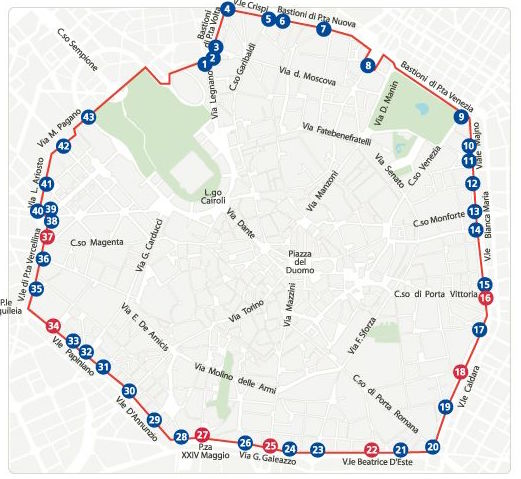
\includegraphics[width=.64\textwidth]{../img/milan-map.jpg}
	\caption{Milan Ecopass/Area C \citep{Rotaris2010}}
	\label{fig:milan-map}
\end{figure}

\begin{table}
\begin{center}
\begin{tabular}{|>{\centering}m{1.8cm}|>{\centering}m{1.8cm}|>{\centering}p{1.8cm}|}
\hline 
Emissions Class & Charge (\euro) \tabularnewline
\hline 
\hline 
1 & 0 \tabularnewline
\hline 
2 & 0 \tabularnewline
\hline 
3 & 2 \tabularnewline
\hline 
4 & 5 \tabularnewline
\hline 
5 & 10 \tabularnewline
\hline 
\end{tabular}
\par\end{center}
\caption{Ecopass prices. Lower classes are less polluting. Class I includes hybrid and electric cars. Class V low-efficiency diesel and buses. \citep{Rotaris2010} }\label{tab:milan-ecopass-prices}
\end{table}

\begin{table}

\begin{center}
\begin{tabular}{|>{\centering}m{2.2cm}|>{\centering}m{1.8cm}|}
\hline 
User Class & Charge (\euro)\tabularnewline
\hline 
\hline 
standard & 5\tabularnewline
\hline 
residents & 2\tabularnewline
\hline 
service & 3\tabularnewline
\hline 
\end{tabular}
\par\end{center}
\caption{Area C prices. ``Service vehicles'' are those enaged in certain commercial activities.}\label{tab:milan-area-c-prices}
\end{table}

\subsection{Results}

During the Ecopass trial, congestion inside the cordon fell by 12.3\%, vehicle-kilometers traveled by 14.2\% and accidents by 20.6\% while bus speeds and private vehicle speeds rose, respectively, 7.8\% and 4\%. Using time-series data during the suspension in summer 2012, \citet{Gibson2015} estimate that the suspension raised entries to the charging zone during charging hours by 27,500 per day (14.5 percent), CO concentrations by 6 percent and PM10 concentrations by 17 percent.

\subsection{Finances}

Revenue and costs are both low. Edoardo Croci, who led the petition drive that resulted in Area C, uses financial reports from the city to report \euro 30 million in revenue for 2013 and 2014 \citep[p. 257]{Croci2016}, although this neglects revenue from fines, which \citet{Rotaris2010} reports were substantial under Ecopass. Costs are less certain. Based on unspecified sources, Croci cites operating costs of \euro 14 million per year and \euro 7 million in implementation cost. Based on unspecified informal press reports, \citet{Rotaris2010} reports \euro 7 million per year in operating cost for Ecopass. The Milan city website for Area C reports 7 million in operating costs for Area C for 2012 (why this should be so much lower than Croci's estimates is unclear), and says net revenues are earmarked for public transport and cycle improvements.\footnote{https://www.comune.milano.it/wps/portal/ist/it/servizi/mobilita/Area\_C/motivazioni} In any case, sources agree that implentation costs were relatively low, because both schemes have used the infrastructure that already existed for the Cerchia dei Bastioni ZTL.

% \citet{Danielis2011} report Ecopass revenues between \euro 10 and 12 million per year and operating costs of about \euro 6.5 million.




